\chapter{Imagenes sobre algunos datos interesantes\label{apendA}}


\begin{figure}[htp]
\centering
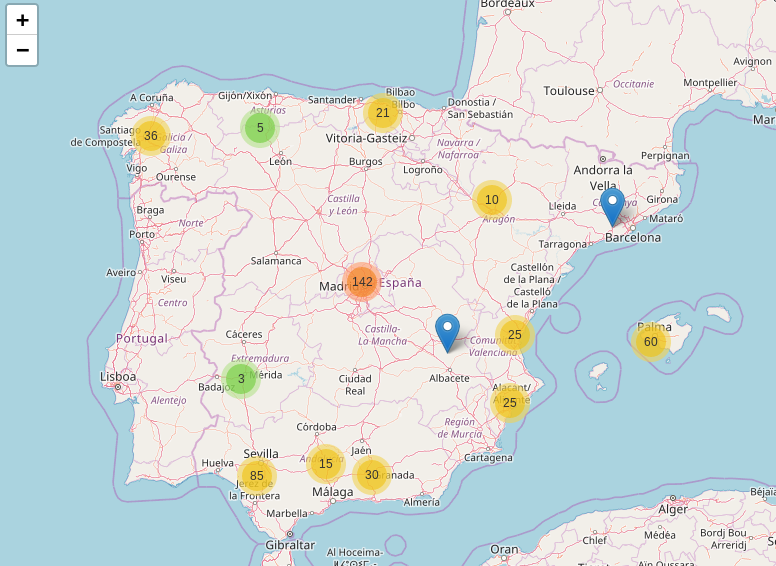
\includegraphics[scale=.50]{Anexos/PuntosNegrosEspana.png}
\caption{Puntos negros de España obtenidos}
\label{blackShapes}
\end{figure}

\begin{figure}[htp]
\centering
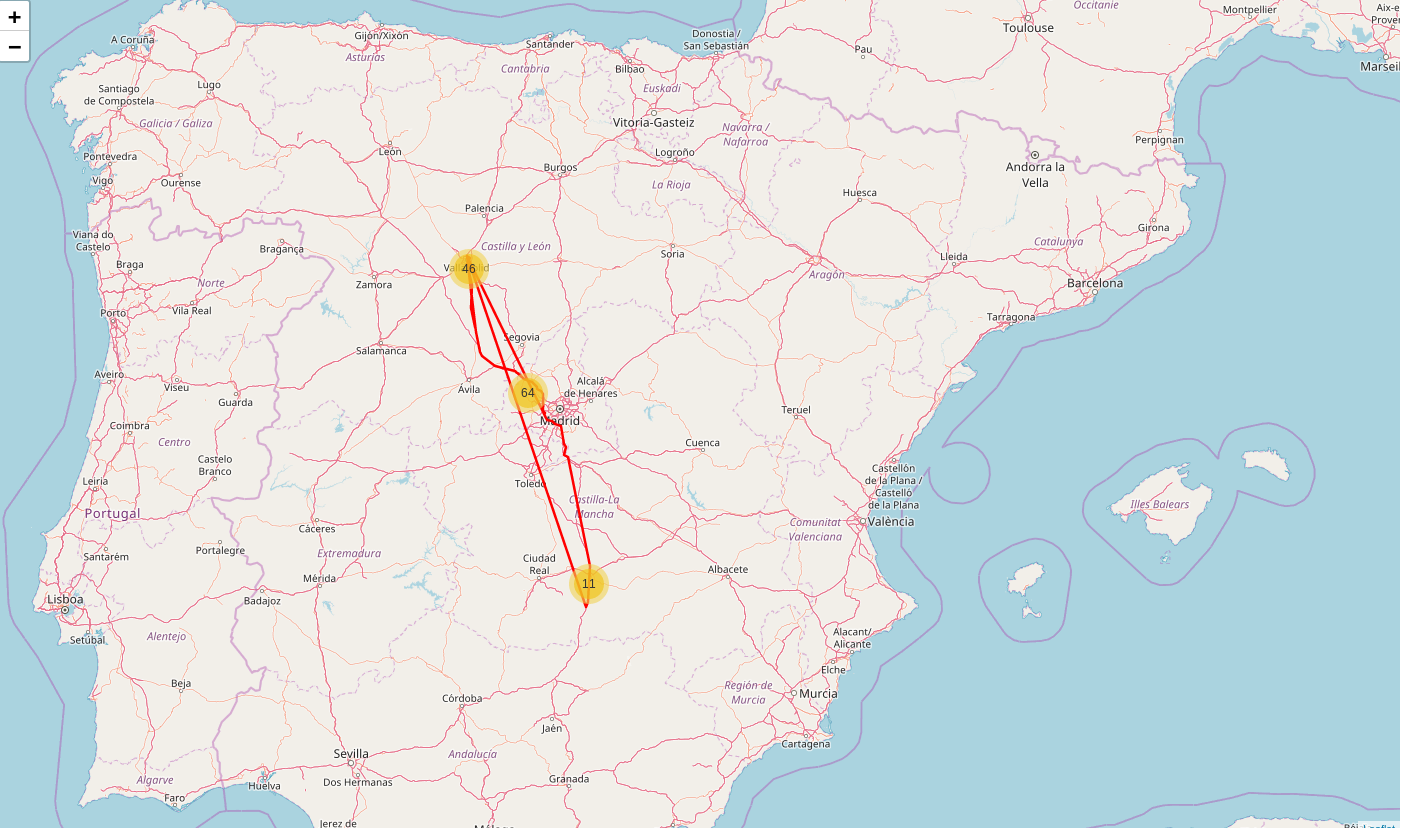
\includegraphics[scale=.30]{Anexos/rutaDeUnVehiculo.png}
\caption{Ruta de un vehiculo}
\label{littleRoute}
\end{figure}


\begin{figure}[htp]
\centering
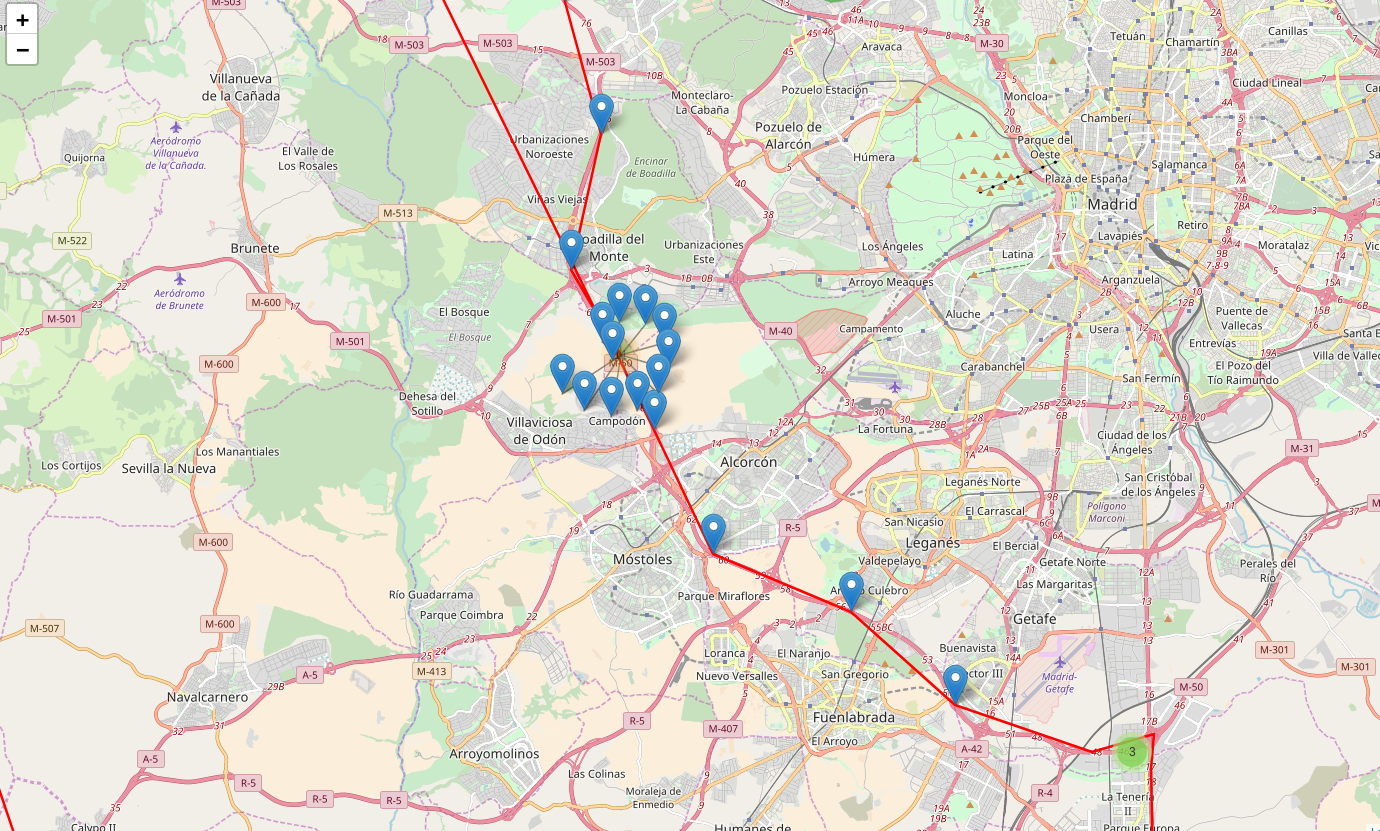
\includegraphics[scale=.30]{Anexos/rutaConParada.png}
\caption{Pequeña ruta y parada de un vehiculo}
\label{littleRouteWithStop}
\end{figure}


\chapter{Script para el API de consultas a MongoDB integrado con OSM\label{apendB}}
\lstinputlisting[language=Python, basicstyle=\scriptsize]{Anexos/mongoUbicationServer.py}

\newpage
\chapter{Script de envio de tramas para la simulación\label{apendC}}
\lstinputlisting[language=Python, basicstyle=\scriptsize]{Anexos/sendTraffic.py}

\newpage
\chapter{Script de SparkSQL Streaming}\label{apendD}
\lstinputlisting[language=Python, basicstyle=\scriptsize]{Anexos/sparkStructStream.py}

\newpage
\chapter{Script de Spark Streaming}\label{apendE}
\lstinputlisting[language=Python, basicstyle=\scriptsize]{Anexos/sparkStreamingWithoutMongo.py}

\newpage
\chapter{Script de SparkSQL Streaming con las consultas a MongoDB}\label{apendF}
\lstinputlisting[language=Python, basicstyle=\scriptsize]{Anexos/sparkStreaming.py}

\newpage
\chapter{Script de creación del índice en Elasticserach}\label{apendG}
\lstinputlisting[language=Python, basicstyle=\scriptsize]{Anexos/CreateIndexForElastic.py}

\newpage
\chapter{Pipe definida para Logstash}\label{apendH}
\lstinputlisting[basicstyle=\small]{Anexos/logstashkafka.conf}


\newpage

\chapter{Pipe definida para Logstash con actualización\label{apendI}}
\lstinputlisting[basicstyle=\scriptsize]{Anexos/logstashkafkaUpdates.conf}


\newpage
\chapter{Pipe definida para Logstash con actualización\label{apendJ}}
\lstinputlisting[basicstyle=\scriptsize]{Anexos/ConsultaTrafico.json}
